\documentclass{article}
\usepackage{tikz}
\usetikzlibrary{arrows.meta}
\usepackage{pgfplots}
\pgfplotsset{compat=1.18}

\begin{document}

\begin{figure}[h]
    \centering
    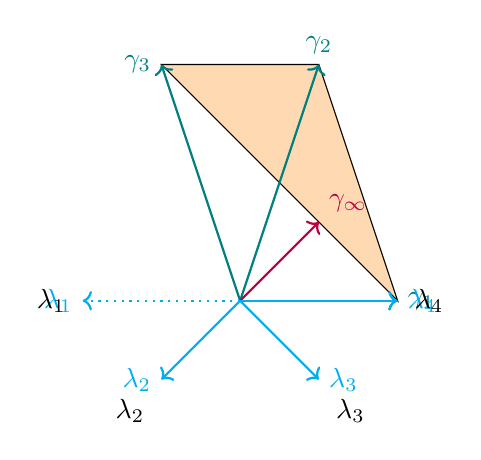
\begin{tikzpicture}[scale=2]
        % Define points
        \coordinate (O) at (0,0);
        \coordinate (A) at (1,0);
        \coordinate (B) at (0.5,1.5);
        \coordinate (C) at (-0.5,1.5);
        
        % Draw the convex hull
        \draw[fill=orange!30] (A) -- (B) -- (C) -- cycle;
        
        % Draw the vectors
        \draw[->, teal, thick] (O) -- (A) node[right] {$\gamma_1$};
        \draw[->, teal, thick] (O) -- (B) node[above] {$\gamma_2$};
        \draw[->, teal, thick] (O) -- (C) node[left] {$\gamma_3$};
        
        % Draw the distance vector
        \draw[->, purple, thick] (O) -- (0.5,0.5) node[above right] {$\gamma_\infty$};
        
        % Draw the lambda vectors
        \draw[->, cyan, dotted, thick] (O) -- (-1,0) node[left] {$\lambda_1$};
        \draw[->, cyan, thick] (O) -- (-0.5,-0.5) node[left] {$\lambda_2$};
        \draw[->, cyan, thick] (O) -- (0.5,-0.5) node[right] {$\lambda_3$};
        \draw[->, cyan, thick] (O) -- (1,0) node[right] {$\lambda_4$};
        
        % Draw the labels for the lambda vectors
        \node at (-1.2,0) {$\lambda_1$};
        \node at (-0.7,-0.7) {$\lambda_2$};
        \node at (0.7,-0.7) {$\lambda_3$};
        \node at (1.2,0) {$\lambda_4$};
    \end{tikzpicture}
    
    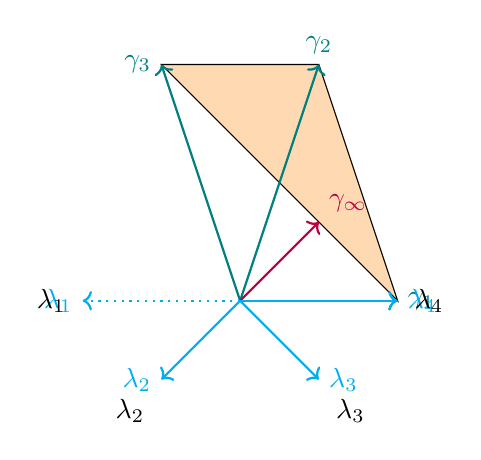
\begin{tikzpicture}[scale=2]
        % Define points
        \coordinate (O) at (0,0);
        \coordinate (A) at (1,0);
        \coordinate (B) at (0.5,1.5);
        \coordinate (C) at (-0.5,1.5);
        
        % Draw the convex hull
        \draw[fill=orange!30] (A) -- (B) -- (C) -- cycle;
        
        % Draw the vectors
        \draw[->, teal, thick] (O) -- (A) node[right] {$\gamma_1$};
        \draw[->, teal, thick] (O) -- (B) node[above] {$\gamma_2$};
        \draw[->, teal, thick] (O) -- (C) node[left] {$\gamma_3$};
        
        % Draw the distance vector
        \draw[->, purple, thick] (O) -- (0.5,0.5) node[above right] {$\gamma_\infty$};
        
        % Draw the lambda vectors
        \draw[->, cyan, dotted, thick] (O) -- (-1,0) node[left] {$\lambda_1$};
        \draw[->, cyan, thick] (O) -- (-0.5,-0.5) node[left] {$\lambda_2$};
        \draw[->, cyan, thick] (O) -- (0.5,-0.5) node[right] {$\lambda_3$};
        \draw[->, cyan, thick] (O) -- (1,0) node[right] {$\lambda_4$};
        
        % Draw the labels for the lambda vectors
        \node at (-1.2,0) {$\lambda_1$};
        \node at (-0.7,-0.7) {$\lambda_2$};
        \node at (0.7,-0.7) {$\lambda_3$};
        \node at (1.2,0) {$\lambda_4$};
    \end{tikzpicture}
\end{figure}

\end{document}